
%-------------------------------------------------------------------------------
%-------------------------------------------------------------------------------
%-------------------------------------------------------------------------------
\chapter{DS1+ X 1997}
%-------------------------------------------------------------------------------
%-------------------------------------------------------------------------------
%-------------------------------------------------------------------------------
%-------------------------------------------------------------------------------
%-------------------------------------------------------------------------------
%-------------------------------------------------------------------------------
\section{Quadtrees}
%-------------------------------------------------------------------------------
%-------------------------------------------------------------------------------
%-------------------------------------------------------------------------------
\begin{Exercise}[title=Propriétés des quadtrees]
\renewcommand{\labelenumi}{\alph{enumi})}
\begin{enumerate}
    \itemsep6mm 
    \item On peut proposer
    
    \begin{center}
        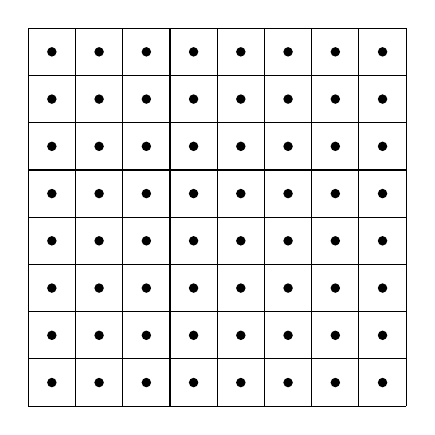
\begin{tikzpicture}[scale = 0.6]
            \foreach\i in {0, 1, ..., 8} {\draw (0, \i) -- (8, \i); \draw (\i, 0) -- (\i, 8);};
            \foreach \i in {0, 1, ..., 7} 
                {\foreach \j in {0, 1, ..., 7} \fill (\i+0.5, \j+0.5) circle (0.1);};
        \end{tikzpicture}
        \hskip 5mm et \hskip 5mm
        \begin{tikzpicture}[scale = 0.6]
            \foreach\i in {1, 2, 4} {\draw (0, 0) rectangle (2*\i, 2*\i); 
                                     \draw (\i, 0) -- (\i, 2*\i); 
                                     \draw (0, \i) -- (2*\i, \i);};
            \fill (0.5, 0.5) circle (0.1);
            \fill (1.5, 0.5) circle (0.1);
        \end{tikzpicture}
    \end{center}
%-------------------------------------------------------------------------------
    \item Un quadtree de profondeur $p$ contient au plus $4^p$ feuilles donc $4^p \ge N$, 
    
    c'est-à-dire $p \ge \lceil\log_4(N)\rceil=f(N)$. 

    Pour tout $p_0$ on peut construire un quadtree à $N_0=4^{p_0}$ corps de profondeur $p_0$ obtenu, comme ci-dessus en subdivisant l'univers en $4^{p_0}$ carrés, chacun contenant un corps ; on a bien $p_0=f(N_0)$.
    
    Mais la question est ambigüe, on peut construire un quadtree à $N_0$ corps de profondeur $p_0$ pour tout $N_0$ tel que $f(N_0) = p_0$. En effet, on a alors $4^{p_0-1}< N_0 \le 4^{p_0}$.
    On construit un quadtree de profondeur $p_0-1$ complet comme ci-dessus et place les $N_0$ corps, entre 1 et 4 par nœud. Comme il y a au moins $4^{p_0-1}+1$ corps on devra subdiviser au moins un nœud et on arrive ainsi à une profondeur de $p_0$.
    
        \begin{center}
        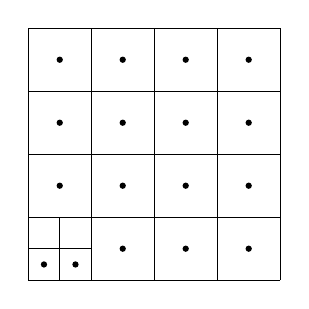
\begin{tikzpicture}[scale = 0.4]
            \foreach\i in {0, 1, ..., 4} {\draw (0, 2*\i) -- (8, 2*\i); \draw (2*\i, 0) -- (2*\i, 8);};
            \foreach \i in {0, 1, ..., 3} 
                {\foreach \j in {0, 1, ..., 3} \fill (2*\i+1, 2*\j+1) circle (0.1);};
            \fill[color = white] (0, 0) rectangle (2, 2);
            \draw (0, 0) rectangle (2, 2);
            \draw (1, 0) -- (1, 2);
            \draw (0, 1) -- (2, 1);
            \fill (0.5, 0.5) circle (0.1);
            \fill (1.5, 0.5) circle (0.1);
        \end{tikzpicture}
        \hskip 1cm
        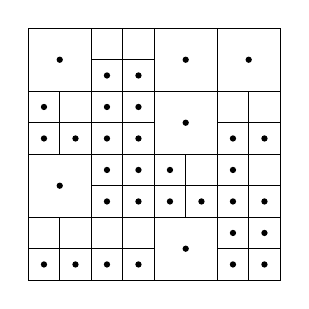
\begin{tikzpicture}[scale = 0.4]
            \foreach\i/\j in {1/3, 1/7, 5/1, 5/5, 5/7, 7/7} 
                {\draw (\i-1, \j-1) rectangle (\i+1, \j+1); 
                 \fill (\i, \j) circle (0.1);};
            \foreach\i/\j in {1/1, 3/1, 3/7, 7/5} 
                {\draw (\i-1, \j-1) rectangle (\i+1, \j+1); 
                 \draw (\i, \j-1) -- (\i, \j+1); 
                 \draw (\i-1, \j) -- (\i+1, \j); 
                 \fill (\i-0.5, \j-0.5) circle (0.1);
                 \fill (\i+0.5, \j-0.5) circle (0.1);};
            \foreach\i/\j in {1/5, 5/3, 7/3} 
                {\draw (\i-1, \j-1) rectangle (\i+1, \j+1); 
                 \draw (\i, \j-1) -- (\i, \j+1); 
                 \draw (\i-1, \j) -- (\i+1, \j); 
                 \fill (\i-0.5, \j-0.5) circle (0.1);
                 \fill (\i-0.5, \j+0.5) circle (0.1);
                 \fill (\i+0.5, \j-0.5) circle (0.1);};
            \foreach\i/\j in {3/3, 3/5, 7/1} 
                {\draw (\i-1, \j-1) rectangle (\i+1, \j+1); 
                 \draw (\i, \j-1) -- (\i, \j+1); 
                 \draw (\i-1, \j) -- (\i+1, \j); 
                 \fill (\i-0.5, \j-0.5) circle (0.1);
                 \fill (\i-0.5, \j+0.5) circle (0.1);
                 \fill (\i+0.5, \j-0.5) circle (0.1);
                 \fill (\i+0.5, \j+0.5) circle (0.1);};
        \end{tikzpicture}
    \end{center}

%-------------------------------------------------------------------------------
    \item À partir d'un quadtree $t_p$ contenant $N$ corps avec $N\ge 2$ et de profondeur $p$, on peut construire un quadtree $t_{p+1}$ de profondeur $p+1$ avec $N$ corps en joignant $t_p$ et 4 nœuds vides. On peut donc construire des quadtrees à $N$ corps de profondeur quelconque : il n'y a pas de majorant fonction de $N$ de la profondeur.
%-------------------------------------------------------------------------------
    \item Dans un quadtree de profondeur $p$ il y a au moins un carré au niveau $p-1$ contenant 2 corps.
    La distance entre deux corps distincts inclus dans ce carré est majorée par la longueur du côté, $\displaystyle \frac {D_{\cal U}}{2^{p-1}}$ d'où, pour le minimum des distances,  $\displaystyle \delta \le \frac {D_{\cal U}}{2^{p-1}}$.
    
    On en déduit $\displaystyle p\le 1 + \log_2\left(\frac{D_{\cal U}}{\delta}\right)$, puis, comme $p$ est entier, $\displaystyle p\le 1 + \left\lfloor\log_2\left(\frac{D_{\cal U}}{\delta}\right)\right\rfloor$.
    
\begin{minipage}{0.6\textwidth}
    Inversement, si on pose $\displaystyle p_0 = 1 + \left\lfloor\log_2\left(\frac{D_{\cal U}}{\delta}\right)\right\rfloor$, 
    
    on a $\displaystyle \frac {D_{\cal U}}{2^{p}}< \delta \le  \frac {D_{\cal U}}{2^{p-1}}$. On peut alors placer deux corps en $(0,0)$ et $(\delta, 0)$ et un quadtree qui les contient devra être de profondeur $p_0$ pour les séparer.
    
    La borne supérieure de la profondeur est bien 
    \[1 + \left\lfloor\log_2\left(\frac{D_{\cal U}}{\delta}\right)\right\rfloor\]
\end{minipage}
\begin{minipage}{0.4\textwidth}
    \begin{center}
        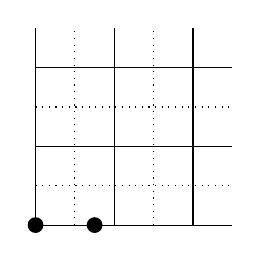
\begin{tikzpicture}[scale = 0.5]
        \foreach \i in {1, 3}
            {\draw[dotted] (\i, 0) -- (\i, 5); \draw[dotted] (0, \i) -- (5, \i);};
        \foreach \i in {0, 2, 4}
            {\draw (\i, 0) -- (\i, 5); \draw (0, \i) -- (5, \i);};
        \fill (0, 0) circle (0.2);
        \fill (1.5, 0) circle (0.2);
        \end{tikzpicture}
    \end{center}
\end{minipage}
%-------------------------------------------------------------------------------
    \item Le plus petit nombre strictement positif représentable est $2^e$ donc
$\delta \ge 2^e$.

Le plus grand nombre représentable est $2^e(2^m-1)$ donc $D_{\cal U} \le 2^e(2^m-1)$.

On en déduit $\displaystyle p\le 1 + \left\lfloor\log_2\left(\frac{D_{\cal U}}{\delta}\right)\right\rfloor \le 1 + \bigl\lfloor\log_2(2^m-1)\bigr\rfloor = m$.
\end{enumerate}
\end{Exercise}
%-------------------------------------------------------------------------------
%-------------------------------------------------------------------------------
%-------------------------------------------------------------------------------
\section{Construction du quadtree}
%-------------------------------------------------------------------------------
%-------------------------------------------------------------------------------
%-------------------------------------------------------------------------------
\begin{Exercise}[title=Opérations élémentaires]
\renewcommand{\labelenumi}{\alph{enumi})}
\begin{enumerate}
   \itemsep6mm 
    \item Ne pas oublier les symboles des opérations sur les flottants.
\begin{lstlisting}
let add v1 v2 = {x = v1.x +. v2.x; y = v1.y +. v2.y};;
\end{lstlisting}

\begin{lstlisting}
let sub v1 v2 = {x=v1.x-.v2.x; y=v1.y-.v2.y};;
\end{lstlisting}
%-------------------------------------------------------------------------------
    \item Même remarque
\begin{lstlisting}
let scal m u  = {x = m*.u.x; y = m*.u.y};;
\end{lstlisting}
%-------------------------------------------------------------------------------
    \item L'exponentiation demande des termes flottants, même pour l'exposant.
\end{enumerate}
let carre u   = u.x**2.0 +. u.y**2.0;;
\end{Exercise}
%-------------------------------------------------------------------------------
%-------------------------------------------------------------------------------
\begin{Exercise}[title=Indices]

On choisit l'ordre suivant
\hskip 3cm
\begin{tikzpicture}[scale = 0.6]
\draw[->] (0, 0) -- (5, 0) node[right] {$x$};;
\draw[->] (0, 0) -- (0, 5) node[left] {$y$};;
\foreach \i in {0, 2, 4}
    {\draw[dotted] (\i, 0) -- (\i, 4); \draw[dotted] (0, \i) -- (4, \i);};
\draw (1, 1) node {0};;
\draw (3, 1) node {1};;
\draw (1, 3) node  {2};;
\draw (3, 3) node {3};;
\end{tikzpicture}

\newpage

\renewcommand{\labelenumi}{\alph{enumi})}
\begin{enumerate}
   \itemsep6mm 
    \item On place les nœuds en fonction de leur position par rapport au centre.
\begin{lstlisting}
let indice_fille p_c p =
    (if p_c.y > p.y then 0 else 2) 
  + (if p_c.x > p.x then 0 else 1);;
\end{lstlisting}
%-------------------------------------------------------------------------------
    \item La taille de la sous-cellule est divisée par 2 et le centre est à la moitié de la taille.
\begin{lstlisting}
let position_fille p_c taille i =
    let t = taille/.4.0 in
    match i with
    | 0 -> add p_c {x =   t; y =   t}
    | 1 -> add p_c {x =   t; y = -.t}
    | 2 -> add p_c {x = -.t; y =   t}
    | _ -> add p_c {x = -.t; y = -.t};;
\end{lstlisting}
Le dernier motif est laissé ouvert pour que le pattern matching soit exhaustif.
\end{enumerate}
\end{Exercise}
%-------------------------------------------------------------------------------
%-------------------------------------------------------------------------------
\begin{Exercise}[title=Arbre-univers]
\renewcommand{\labelenumi}{\alph{enumi})}
\begin{enumerate}
   \itemsep6mm 
    \item Si on insère dans un arbre vide, on obtient une feuille,

si on insère dans une feuille, on crée un Noeud et on place le nouveau corps, ainsi que celui qui était dans la feuille, le centre est donné par le vecteur reçu,

si on insère dans un nœud, on insère dans le fils correspondant, on transmet la nouvelle position du centre.

On commence par une fonction qui factorise l'ajout d'un corps dans un tableau, elle sert 3 fois.
\begin{lstlisting}
let rec insere_corps corps arbre p_c taille = 
    let ajoute corps filles centre taille =
      let k= indice_fille p_c corps.pos in
      let new_c = position_fille p_c taille ind in
      let t = taille /. 2.0 in
      filles.(k) <- insere_corps corps filles.(k) new_c t in
    match arbre with
   | Vide -> Feuille(corps)
   | Feuille(c) -> let filles = Array.make 4 Vide in
      ajoute c filles p_c taille;
      ajoute corps filles p_c taille;
      Noeud({cm_mass = 0.0; 
             cm_pos = vecteur_nul; 
             filles = filles})
   | Noeud(cellulle) ->
      ajoute corps cellulle.filles p_c taille;
      arbre;;
\end{lstlisting}
%-------------------------------------------------------------------------------
    \item On suppose que tous les corps à insérer ont des positions appartenant au carré $[-{\cal D}_{\cal U}; {\cal D}_{\cal U}]^2$.
   
   On suppose aussi que les positions des corps à insérer sont distinctes et, de plus, séparées au sens de la norme introduite en {\bf 1.d)} d'au moins $2^{e}$, voir le {\bf 1. e)}. 
   
   Pour démontrer la terminaison, on va aussi prouver l'algorithme en ce sens qu'il place les corps géométriquement dans des carrés qui les contiennent. On considère la propriété suivante :
   
    \begin{itemize}
        \item pour tout arbre ne contenant que des corps dont les positions sont dans le carré 
        
        $[\type{p\_c - taille/2; p\_c + taille/2}]^2$,
        \item pour tout corps \type{corps} de position dans le carré $[\type{p\_c - taille/2; p\_c + taille/2}]^2$,
        \item l'appel de \type{insere\_corps corps arbre p\_c taille} termine.
    \end{itemize}
    
    Le résultat de l'appel fournira un arbre qui, lui aussi, ne contient que des corps dont les positions sont dans le carré $[\type{p\_c - taille/2; p\_c + taille/2}]^2$.
    \newpage
    
    On démontre la propriété par induction structurelle.
    
\begin{itemize}
\item Si l'arbre est vide, la fonction construit une feuille et termine.
\item Si l'arbre est une feuille, celle-ci contient un unique corps. L'algorithme construit un nœud et place ce corps dans une des branches en remplaçant une fille vide. Il place alors le nouveau corps
 
    soit dans une autre branche et l'algorithme termine,
    
    soit dans la même branche  avec une taille diminuée de moitié. Cette situation ne peut que se reproduire qu'un nombre fini de fois car sinon, on parviendrait à une taille strictement majorée par $2^e$ et deux corps dans un carré de côté $c < 2^e$ ce qui a été supposé impossible.
    
    L'algorithme termine.
\item Si \type{arbre} est un nœud, on suppose que l'algorithme termine si on l'applique aux filles.

\type{indice\_fille} et \type{position\_fille} sélectionnent la bonne cellule fille et la fonction \type{ajoute} effectue un appel récursif sur l'une des filles donc termine.
\end{itemize}
%-------------------------------------------------------------------------------
    \item La fonction \type{insere\_corps} effectue un nombre fini d'opérations car elle suit une branche de l'arbre puis, eventuellement prolonge une branche mais la profondeur maximale est bornée d'après la question {\bf 1. e)}.
   
   La complexité de l'insertion de $N$ corps est donc linéaire en $N$.
\end{enumerate}
\end{Exercise}
%-------------------------------------------------------------------------------
%-------------------------------------------------------------------------------
%-------------------------------------------------------------------------------
\section{Calculs des forces}
%-------------------------------------------------------------------------------
%-------------------------------------------------------------------------------
%-------------------------------------------------------------------------------
\begin{Exercise}[title=Barycentres]
La fonction auxiliaire calcule la masse et la somme des positions récursivement et on modifie l'arbre.

On calcule la somme plutôt que le barycentre pour ne pas avoir à re-multiplier par les masses.

Comme on veut un résultat \type{unit}, l'appel final doit être encapsulé.
\begin{lstlisting}
let barycentres arbre =
  let rec masse_somme arbre =
    match arbre with
    |Vide -> (0.0, vecteur_nul)
    |Feuille(c) -> (c.mass, scal c.mass c.pos)
    |Noeud(cellule) 
          -> let m = ref 0.0 and s = ref vecteur_nul in
             for i = 0 to 3 do
                let mi, si = masse_somme cellule.filles.(i) in
                m := !m +. mi;
                s := add !s si done;
             cellule.cm_mass <- !m;
             cellule.cm_pos <- scal (1.0 /. !m) !s;
             !m, !s
  in let _ = masse_somme arbre in ();;
\end{lstlisting}
\end{Exercise}
%-------------------------------------------------------------------------------
%-------------------------------------------------------------------------------
\begin{Exercise}[title=Gravitation]
\renewcommand{\labelenumi}{\alph{enumi})}
\begin{enumerate}
   \itemsep6mm 
    \item On commence par un calcul de la distance entre deux points et un calcul du vecteur accélération, si la distance entre les corps est nulle, c'est qu'on cherche l'accélération d'un corps sur lui-même, elle est nulle.
\begin{lstlisting}
let distance a b =
   let vec = sub a b in
   (carre vec)**0.5 ;;
\end{lstlisting}

\newpage

\begin{lstlisting}
let accel point orig masse =
   let vec = sub orig point in
   let r = distance point orig in
   if r = 0.0
   then vecteur_nul
   else scal (masse /. r**3.0) vec;;
\end{lstlisting}
\begin{lstlisting}
let rec grav_approx pos arbre taille = 
   match arbre with
   |Vide -> vecteur_nul
   |Feuille(c)  -> accel pos c.pos c.mass
   |Noeud(cl) 
     -> let r = distance pos cl.cm_pos in 
        if taille < r *. theta
        then accel pos cl.cm_pos cl.cm_mass
        else begin
            let acc = ref vecteur_nul 
            and t = taille /. 2.0 in
            for i=0 to 3 do 
                acc := add !acc 
                           (grav_approx pos cl.filles.(i) t) 
            done;
            !acc end ;;
\end{lstlisting}
%-------------------------------------------------------------------------------
    \item Le barycentre peut se situer en tout point du carré.
    
    \begin{minipage}{0.5\textwidth}
Pour qu'une cellule de taille $D$ soit subdivisée, il faut que son centre de masse soit situé à une distance inférieure à $\frac D\theta$ du corps $c$ ; cette cellule doit donc être entièrement inclus dans le disque de centre $c$ et de rayon $\frac D\theta + D\sqrt2$. Comme toutes les cellules de même taille sont deux à deux disjointes, la somme des aires des cellules divisables est majorée par l'aire du disque d'où, si $N$ est le nombre de ces cellules, 

 $\displaystyle N.D^2 \le \pi \left(\frac D\theta + D\sqrt2\right)^2$. 
 
 Le nombre est donc majoré par
\[K(\theta)= \pi \left(\frac 1\theta + \sqrt2\right)^2\]
\end{minipage}
\begin{minipage}{0.5\textwidth}
    \begin{center}
        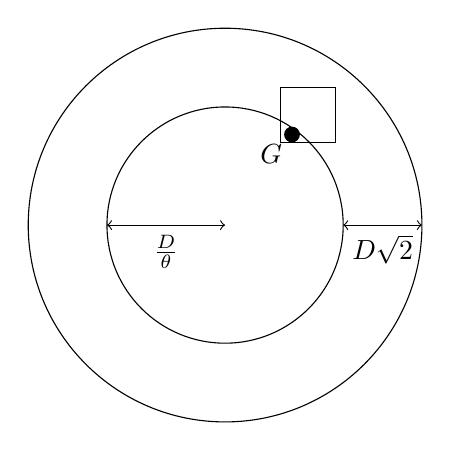
\begin{tikzpicture}[scale = 0.5]
        \draw (0, 0) circle (3);
        \draw (0, 0) circle (5);
        \draw (1.4, 2.1) rectangle (2.8, 3.5);
        \draw[<->] (0, 0) -- node[below]{$\frac D\theta$} (-3, 0);
        \draw[<->] (3, 0) -- node[below]{$D\sqrt 2$} (5, 0);
        \fill (1.7, 2.3) circle (0.2) node [below left]{$G$};
        \end{tikzpicture}
    \end{center}
\end{minipage}

%-------------------------------------------------------------------------------
    \item  Un appel \type{grav\_approx c arbre taille} engendre au plus $K(\theta)$ appels récursifs pour des nœuds de taille $2^{-k}\times$ \type{taille} pour tout entier $k$ d'après la question ci-dessus. Comme  la profondeur de l'arbre est majorée par $m$, le nombre total d'appels est majoré par $mK(\theta)$ qui est une constante. Pour $N$ points la complexité est donc un ${\cal O}(n)$.
%-------------------------------------------------------------------------------
\end{enumerate}
\end{Exercise}
%-------------------------------------------------------------------------------
%-------------------------------------------------------------------------------


% Un appel ?grav_approx c arbre t? gén{\`e}re au plus $K(\theta)$ appels
% ?grav_approx c arbre' (t/2^k)? pour tout entier $k$ d'apr{\`e}s ce qui préc{\`e}de
% et la profondeur de l'arbre étant majorée par $m$, le nombre total d'appels
% à ?grav_approx? générés est majoré par $mK(\theta)$ qui est une constante.
% Chacun de ces appels effectue, hors appels récursifs, un nombre borné
% d'opérations, donc la complexité de ?grav_approx? est bornée et celle de
% ?ajuste_approx? est un $O(N)$.
% \SV
% \centerline{\bf Programmes en Pascal}
% \sv
% Les prototypes des fonctions demandées ne sont pas tous conformes à la syntaxe
% du Pascal en vigueur dans les classes préparatoires~:
% une fonction ne peut retourner un résultat non scalaire et les descriptions
% de type dans une en-tête de procédure ou de fonction
% (?function cree_feuille(c:1..N):arbre?) ne sont pas autorisées, il faut
% donner un nom au type ?1..N?.
% Ces restrictions ne sont pas supportées par tous les compilateurs Pascal,
% en particulier le traducteur ?p2c? de la Free Software Foundation a permi
% de compiler avec succ{\`e}s toutes les procédures et fonctions qui suivent.

% %-------------------------------------------------------------------------------
% \q{2abc}
% ?
%   procedure add(u,v : vecteur; var r: vecteur);
%   begin
%      r.x := u.x + v.x;
%      r.y := u.y + v.y
%   end;
    
%   procedure sub(u,v: vecteur; var r: vecteur);
%   begin
%      r.x := u.x - v.x;
%      r.y := u.y - v.y
%   end;
    
%   procedure scal(m: real; u: vecteur; var r: vecteur);
%   begin
%      r.x := m*u.x;
%      r.y := m*u.y
%   end;
    
%   function carre(u : vecteur): real;
%   begin
%      carre := u.x*u.x + u.y*u.y
%   end;
% ?
% %-------------------------------------------------------------------------------
% \q{3ab}
% ?
%   function indice_fille(p_c,p: vecteur): integer;
%   var res: integer;
%   begin
%      if p_c.y > p.y then res := 1 else res := 0;
%      if p_c.x > p.x then res := res + 2;
%      indice_fille := res
%   end;
  
%   function position_fille(p: vecteur; taille: real; i: integer): vecteur;
%   var t: real; v: vecteur;
%   begin
%      t := taille/4.0;
%      if i >= 2 then v.x := -t else v.x := t;
%      if odd(i) then v.y := -t else v.y := t;
%      add(p,v,v);
%      position_fille := v
%   end;
% ?
% %-------------------------------------------------------------------------------
% \q{4a}
% ?
%   procedure insere_dans_filles(c: 1..N; var a: arbre; p: vecteur; taille: real);
%   forward;
    
%   procedure insere_corps(c: 1..N; var a: arbre; p: vecteur; taille: real);
%   var b: arbre;
%   begin
%      if a = nil then a := cree_feuille(c)
%      else if a^.nature = Noeud then insere_dans_filles(c,a,p,taille)
%      else begin
%         b := cree_noeud(0.0,vecteur_nul,nil,nil,nil,nil);
%         insere_dans_filles(a^.corps,b,p,taille);
%         insere_dans_filles(c,b,p,taille);
%         dispose(a);
%         a := b
%      end
%   end;
    
%   procedure insere_dans_filles;
%   var i: integer; q: vecteur;
%   begin
%      i := indice_fille(p,univers[c].pos);
%      q := position_fille(p,taille,i);
%      insere_corps(c,a^.filles[i],q,taille/2)
%   end;
% ?
% %-------------------------------------------------------------------------------
% \q{5}
% ?
%   procedure mass_pos(a: arbre; var m: real; var pos: vecteur);
%   var i: integer;
%      mi: real;
%   posi: vecteur;
%   begin
%      if a=nil then begin m := 0.0; pos := vecteur_nul end
%      else if a^.nature = Feuille then begin
%         m := univers[a^.corps].mass;
%         scal(m,univers[a^.corps].pos,pos)
%      end
%      else begin
%         m := 0.0;
%         pos := vecteur_nul;
%         for i:=0 to 3 do begin
%           mass_pos(a^.filles[i],mi,posi);
%           m := m + mi;
%           add(pos,posi,pos)
%         end;
%         a^.cm_mass := m;
%         scal(1.0/m,pos,a^.cm_pos)
%      end
%   end;
  
%   procedure barycentres(a: arbre);
%   var m : real;
%      pos: vecteur;
%   begin
%      mass_pos(a,m,pos)
%   end;
% ?
% %-------------------------------------------------------------------------------
% \q{6a}
% ?
%   procedure distance(a,b: vecteur; var r: real; var d: vecteur);
%   begin
%      sub(a,b,d);
%      r := sqrt(carre(d))
%   end;
  
%   function accel(a,b: vecteur; m: real): vecteur;
%   var r : real;
%      d  : vecteur;
%   begin
%      distance(b,a,r,d);
%      scal(m/r/r/r,d,d);
%      accel := d
%   end;
     
%   function grav_approx(pos: vecteur; a: arbre; taille: real): vecteur;
%   var r,t: real;
%         p: vecteur;
%         i: integer;
%   begin
%      if a=nil then grav_approx := vecteur_nul
%      else if a^.nature = Feuille then begin
%         if pos = univers[a^.corps].pos then grav_approx := vecteur_nul
%         else grav_approx := accel(pos,univers[a^.corps].pos,univers[a^.corps].mass)
%      end
%      else begin
%         distance(pos,a^.cm_pos,r,p);
%         if taille < r*theta
%         then grav_approx := accel(pos,a^.cm_pos,a^.cm_mass)
%         else begin
%           t := taille/2.0;
%           p := vecteur_nul;
%           for i:= 0 to 3 do add(p,grav_approx(pos,a^.filles[i],t),p);
%           grav_approx := p
%         end
%      end
%   end;
% ?